\documentclass[tikz,border=10pt]{standalone}
\begin{document}
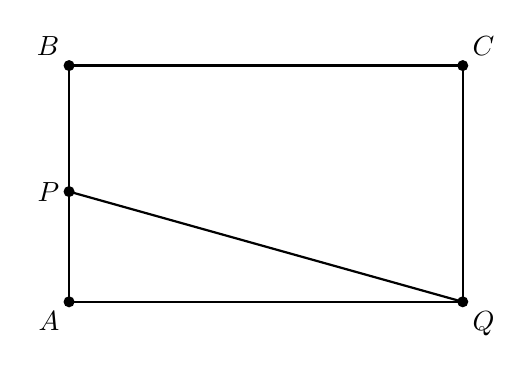
\begin{tikzpicture}
\coordinate (A) at (0,0);
\coordinate (B) at (0,3);
\coordinate (C) at (5,3);
\coordinate (Q) at (5,0);
\coordinate (P) at (0,1.4);

\draw[thick] (A) -- (B) -- (C) -- (Q) -- cycle;
\draw[thick] (P) -- (Q);

\foreach \p in {A,B,C,Q,P}
  \fill (\p) circle (2pt);

\node[above left] at (B) {$B$};
\node[above right] at (C) {$C$};
\node[below left] at (A) {$A$};
\node[below right] at (Q) {$Q$};
\node[left] at (P) {$P$};
\end{tikzpicture}
\end{document}
